\setlength{\parindent}{0pt}
\setlength{\parskip}{0.6em}

%----------------------------------------------------------------------------
\chapter{Architecture plan}
\label{sec:archPlan}
%----------------------------------------------------------------------------

After a research and the first POC, I designed an architecture for the system. I considered all the use cases, the technical nature of the platform and technologies.

\section{Complex architecture}

My first architecture design was a scalable, optimized complex architecture. The \ref{fig:comp_arch} figure shows this architecture.

\begin{figure}[h]
    \centering
    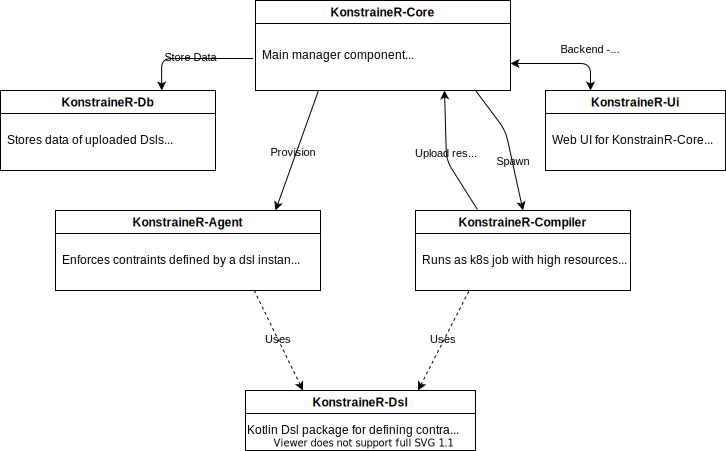
\includegraphics[width=130mm, keepaspectratio]{content_real/25_archPlan/xarch.png}
    \caption{Complex architecture plan}
    \label{fig:comp_arch}
\end{figure}

The main component in this setup is the KonstraineR-Core. This is an HTTP API server managing the whole application. It serves as a store for the uploaded and compiled DSL instances. It handles all tasks related to spawning, starting, configuring, and destroying agents. Most importantly it manages the TLS certificates and webhooks. 

In Kubernetes, webhooks need to communicate with the Kubernetes API on a secured connection. To achieve this, KonstraineR-Agent instances require a TLS certificate, and need to server request on the HTTPS protocol. This certificate can be self signed, but in the webhook creation request the CA Key of the certificate must be sent to the Kubernetes API for signing. After this, the Kubernetes API will trust the certificate of the webhook.

The mutating or validation webhooks have their own Kubernetes resource. It is either a \emph{MutatingWebhookConfiguration} or a \emph{ValidatingWebhookConfiguration}. These need to be created in the cluster, so Kubernetes can send the object creation requests to the Pod implementing the webhook.


